\chapter{Multi-objective optimization}
\label{chapter:multiobjective}
\index{Multi-objective optimization}
In this chapter, the principles of multi-objective optimization are outlined and basic concepts are formally defined.

\section{Basic concepts}
Multi-objective optimization is needed whenever there are several conflicting objectives functions to be optimized simultaneously.

We present the formulation of a multi-objective optimization problem as
\begin{equation}
\label{fun:mop}
\begin{split}
&\text{minimize} \quad \{ f_{1}(x), f_{2}(x),..., f_{k}(x) \} \\
&\text{subject to} \quad x \in S \subset \mathbb{R}^{n}
\end{split}
\end{equation}
with $k\geq 2$ conflicting objective functions $f_{i}: S \rightarrow \mathbb{R} $ and where $x$ is a vector of continuous decision variables from the feasible set $S$. We can denote an objective vector by $z = f(x) = (f_{1}(x), f_{2}(x),..., f_{k}(x))^{T}$.  
If an objective function $ f_{i}$ is to be maximized, this is equivalent to considering minimization $-f_{i}$.

In multi-objective optimization, our aim is to optimize the values of several objectives at the same time however, usually there exist no single point within the search space where all the objectives reach their individual optima. In other words, if we want to gain something, we must give away something else.

In general, problem (\ref{fun:mop}) has many optimal solutions with different trade-offs. These optimal solutions are called Pareto optimal solutions, the so-called Pareto optimal solutions forming a Pareto optimal set. With the goal of being more specific, in (\ref{fun:mop}), a design variable vector $ x^{'} \in S$ and the corresponding objective vector $z$
 are called Pareto optimal if there does not exist another $ x \in S$ such as $f_{i}(x) \leq f_{i}(x^{'})$ for all $i = 1,...,k$ and $f_{j}(x) < f_{j}(x^{'})$ for at least one index $j$.
Therefore, a set of all Pareto optimal solution in $S$ is called a Pareto optimal set and the image of the Pareto optimal set in $f(S)$ is called a Pareto optimal front as shown Figure \ref{fig:decisions_objective_space}
 \begin{figure}[H] %t
	\centering 
	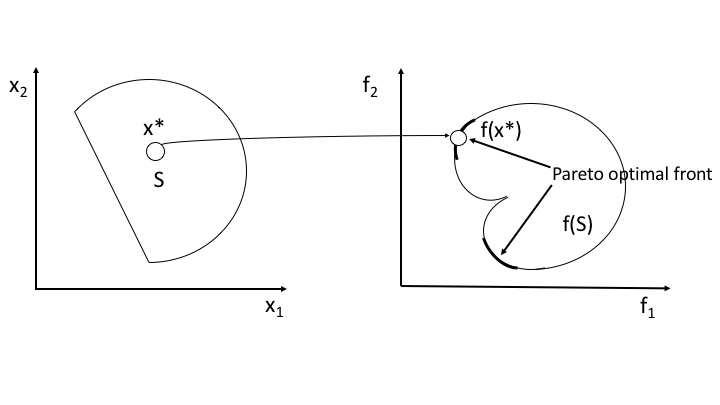
\includegraphics[width=0.80\textwidth]{figures/multiobjective/decision_objective_spaces.png}
	%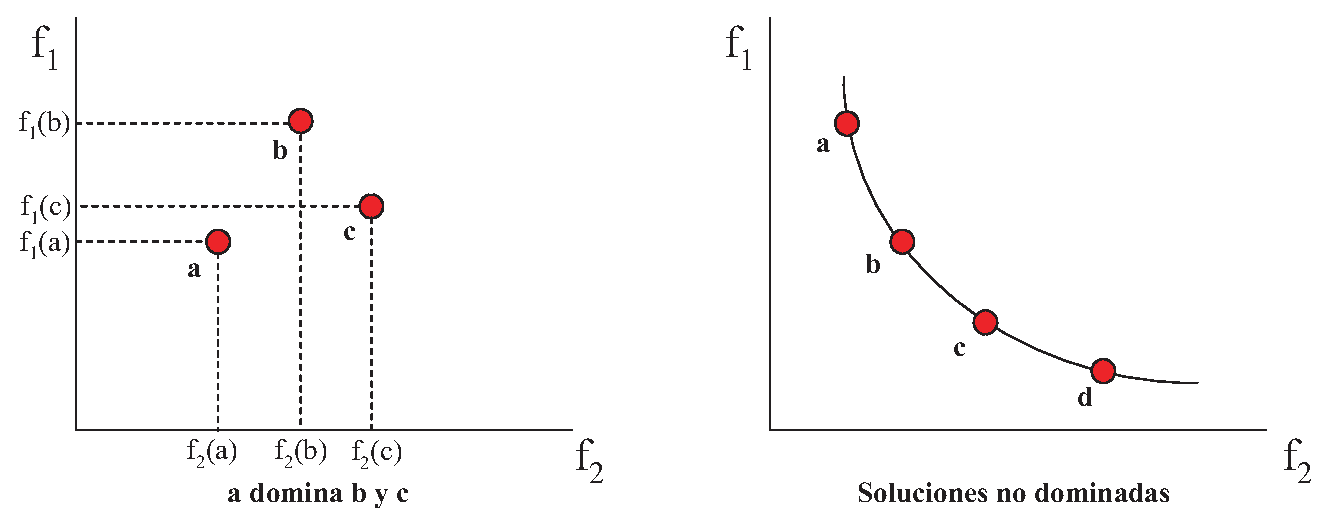
\epsfig{file=./img/metaheuristics/dominancia, width=14cm}
	\caption{Pareto dominance example.} \label{fig:decisions_objective_space}
\end{figure} 
The precedent definition applies for global Pareto optimality however, also local Pareto optimality may be defined. A decision vector $x^{*} \in S$ is locally Pareto optimal if there exists a neighborhood $N(x^{*})$ of $x^{*}$ such that $x^{*}$ is Pareto optimal in $N(x^{*}) \cap S$. The objective vector $f(x^{*})$ is locally Pareto optimal if the corresponding point $x^{*}$ is locally Pareto optimal.
 
The concept of dominance is related to Pareto optimality. In \ref{fun:mop}, an objective vector $z^{1}$ is said to \textit{dominate} another vector $z^{2}$ if $z_{i}^{1} \leq z_{i}^{2} $ for all $i= 1,...,k$, and the inequality is strict for least on index $i$.Furthermore, an objective vector $z^{1}$ is \textit{non-dominated} if there does not exist another objective vector $z^{2}$ such $z^{2}$  dominates $z^{1}$, therefore, Pareto optimal points are non-dominate points. Figure \ref{fig:dominance} shows the concepts of dominance and non-dominance.
\begin{figure}[H] %t
	\centering 
	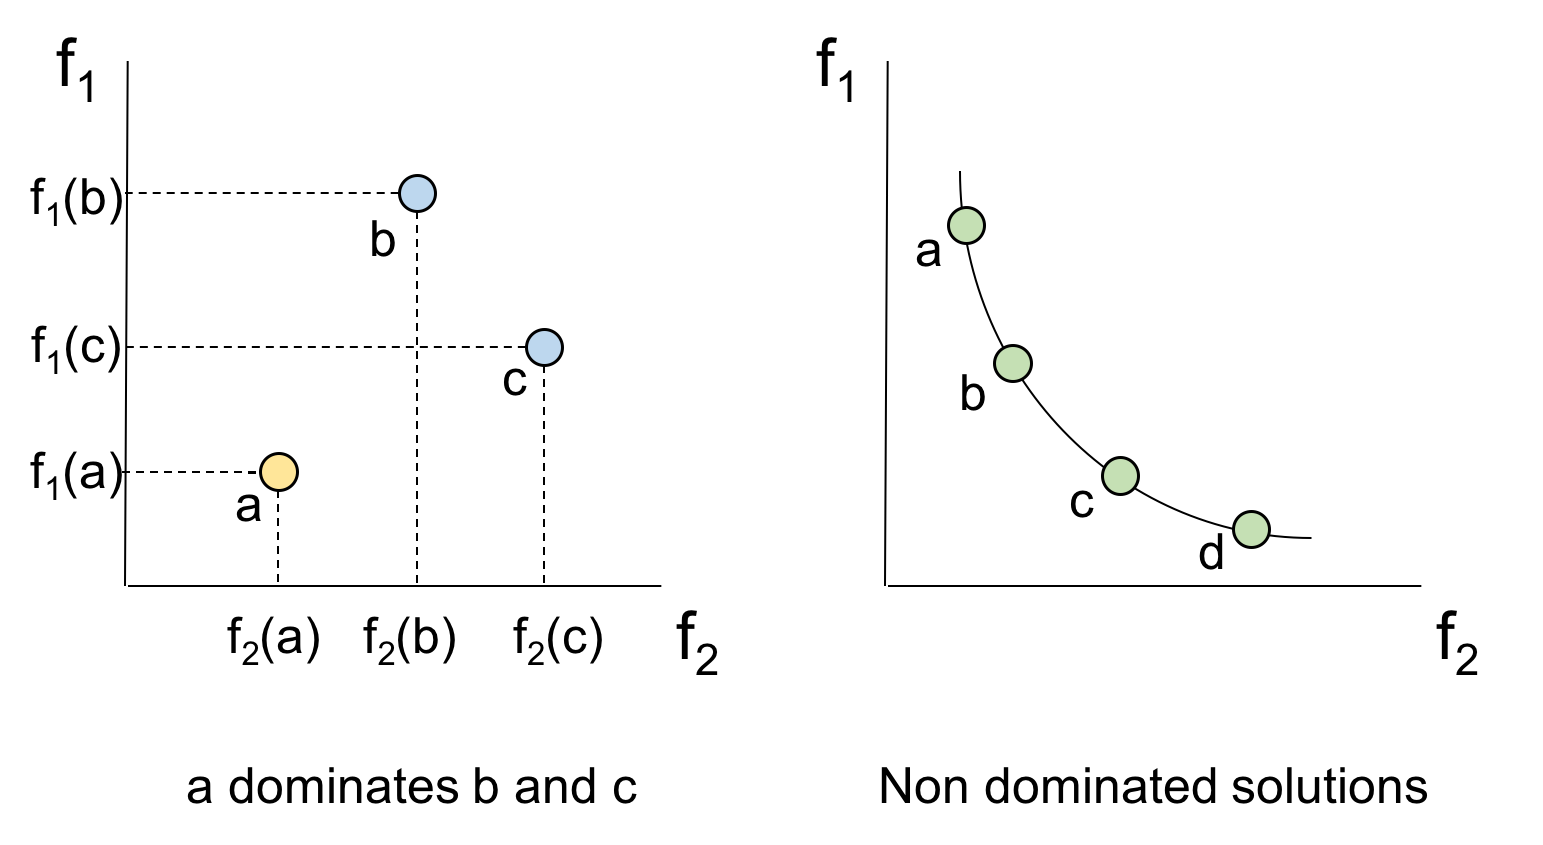
\includegraphics[width=0.80\textwidth]{figures/metaheuristics/my-dominance.png}
	%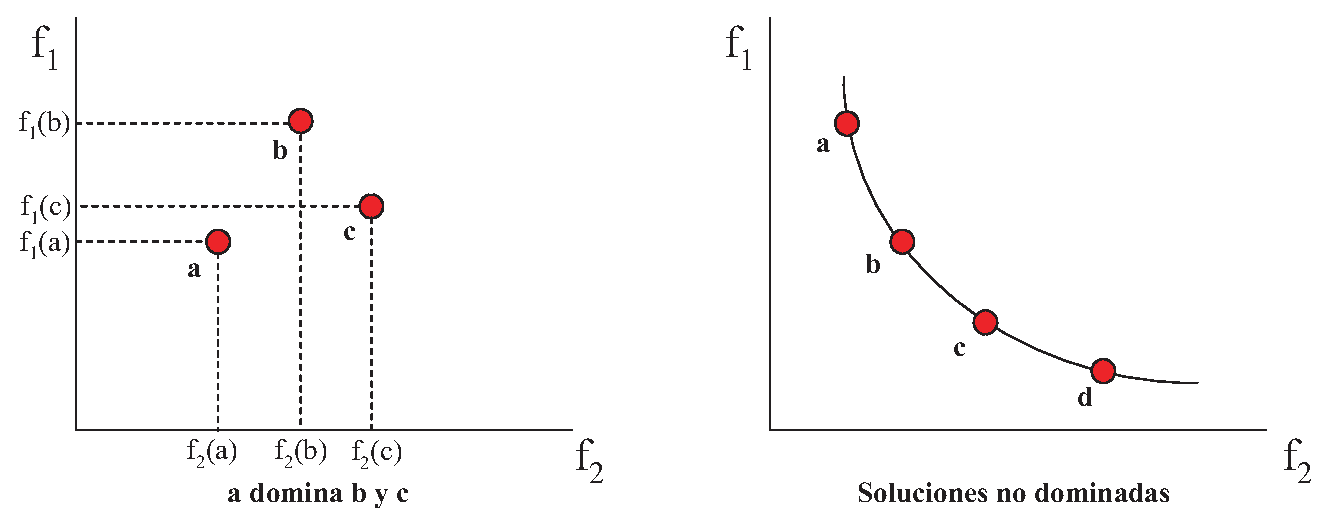
\epsfig{file=./img/metaheuristics/dominancia, width=14cm}
	\caption{Pareto dominance example.} \label{fig:dominance}
\end{figure} 

The limits of objective function values in the Pareto optimal front (called Pareto front) are defined by \textit{ideal} and \textit{nadir} objective vectors. An ideal objective vector $z^{*} \in \mathbb{R}^{k}$ gives lower bounds for the objective functions, and it is obtained by minimizing each objective function individually subject to the constraints. A vector strictly better than $z^{*}$ can be called a\textit{utopian objective vector} $z^{**}$ therefore thus, we set $z_{i}^{**} = z_{i}^{*}- \epsilon$ for $i = 1,...,k$, where $\epsilon$ is a small positive integer. Finally, a \textit{nadir objective vector} $z^{nad}$ is the upper bounds of objective function values in the Pareto optimal set, it is not easy to calculate; consequently, these values are usually only approximated for instance, by using pay-off tables \cite{deb2010nadir,miettinen1999nonlinear}. Examples of ideal, utopian and nadir objective vectors are shown in Figure \ref{fig:ideal_nadir}. Since there exist many Pareto optimal solutions, a decision maker is needed for choosing one solution among them. A decision maker (DM) is a person who is an expert in the domain of the multi-objective optimization problem and can express her/his preference information to choose the most preferred solution.
A very popular type of preference articulation in multi-objective methods is based on \textit{reference points} \cite{branke2008multiobjective,kaisa2016}, which represent the region of interest in the form of desirable objective function values. A reference point is regarded as an intuitive way to express preferences. However, such methods are regarded as ad hoc methods, i.e., methods where the DM cannot be replaced by a value function~\cite{miettinen1999nonlinear,Stewart2005}. 

\begin{figure}[H] %t
	\centering 
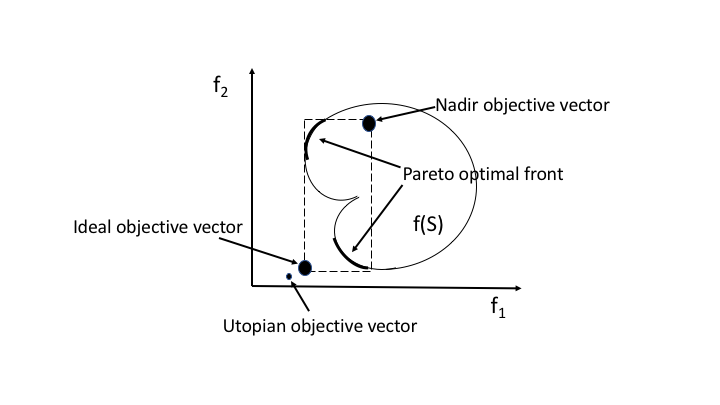
\includegraphics[width=0.80\textwidth]{figures/multiobjective/vector_ideal_nadir.png}
	%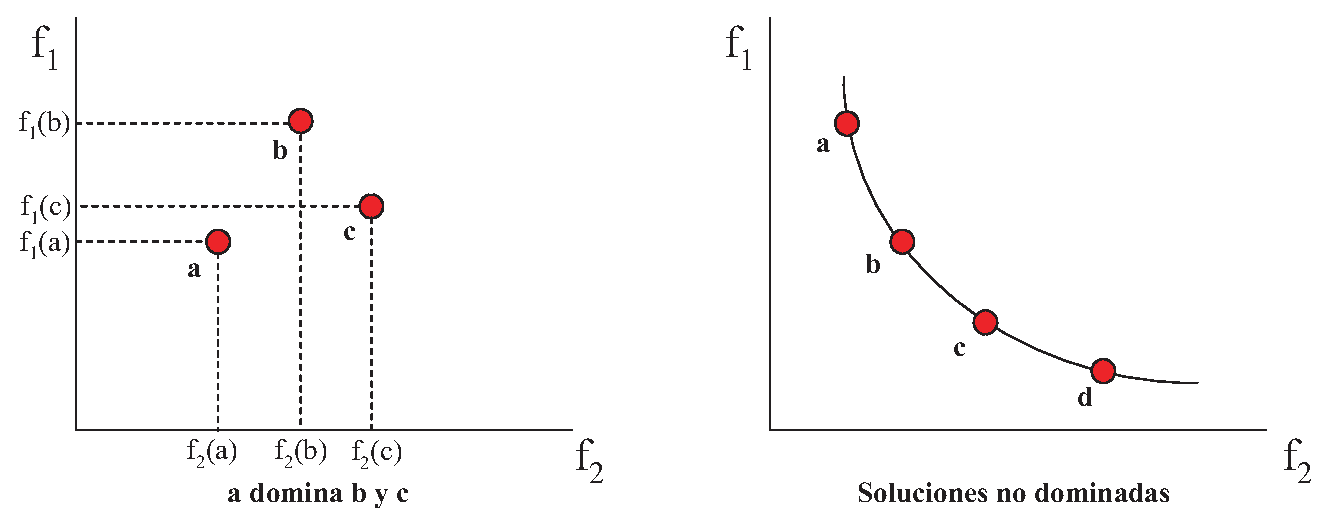
\epsfig{file=./img/metaheuristics/dominancia, width=14cm}
	\caption{Ideal, utopian and nadir objective vectors} \label{fig:ideal_nadir}
\end{figure} 

\section{Classification of multi-objective methods}
The techniques used to solve MOPs are not usually restricted to finding a single solution, but a set of compromise solutions between the multiple conflicting objectives, since there is usually no solution that simultaneously optimizes all objectives. Two stages can therefore be distinguished when addressing this type of problem: on the one hand, the optimization of several objective functions involved and, on the other hand, the decision-making process on which compromise solution is most appropriate \cite{coello07evolutionary}. Multi-objective optimization methods can be classified according to the role of the decision maker in the solution process.  \cite{cohon75review}:

\begin{itemize}
	\item \emph{No-preference methods}: This methods are usually used when there is no DM available or when no preference information from the DM us available consequently, the opinions of the DM are not taken into consideration.
	\item \emph{A posteriori methods}: In this methods the exploration is made as wide as possible to generate as many compromise solutions as possible. It is, then, when the decision-making process by the expert takes place. Precisely, because of this approach, these \emph{a posteriori} techniques are being used in the field of metaheuristics and, particularly, in the field of evolutionary computing \cite{coello07evolutionary, deb01multiobjective}. More specifically, the most advanced algorithms apply \emph{a posteriori} techniques based on the concept of \emph{Pareto Optimality} \cite{pareto96cours}.
	\item \emph{A priori methods}: In this methods, the DM specifies his/her preferences before the solution process. The main withdraw of this method is that DM does not necessarily know beforehand whether the solutions will be realistic. Lexicographic ordering \cite{fishburn1974exceptional} and goal programming \cite{charnes1977goal,charnes1955optimal} are examples of a priori methods.
    \item \emph{Interactive methods}: In interactive methods, the DM articulates preference information iteratively and thus directs the solution process progressively.Only part of the Pareto optimal set has to be generated and evaluated, and based on this data the DM can further adjust his/her preferences as the solution process continues. The procedure is iterated until the DM is satisfied with the Pareto optimal solution. The advantage of using interactive methods is that the DM can guide the solution process and simultaneously learn about the different trade-offs between different solutions. In the last decades, many interactive methods have been proposed such as, Step method \cite{benayoun1971linear}, reference point method \cite{wierzbicki1980use}, satisficing trade-off method \cite{nakayama1984satisficing}, NIMBUS method \cite{miettinen1995interactive}, etc. Recently, several evolutionary algorithm based interactive methods have also proposed, such as progressively interactive evolutionary multi-objective algorithm \cite{deb2010interactive,nebro2018indm2,fowler2010interactive,phelps2003interactive} or interactive territory defining evolutionary algorithm \cite{koksalan2010interactive}.
\end{itemize}

There exists other ways for classifying the multi-objective methods, such as 


-algoritmos dinamicos vs algoritmos estaticos
-hablar de metaheuristics


   